\section{Projektive Geometrie}

\subsection{Homogener Vektor}

$\vec{r} = \begin{bmatrix}
    x_1 \\
    x_2 \\
    x_3 \\
\end{bmatrix}$
\textit{Homogener 2D Vektor} \\

$(x,y) = (\frac{x_1}{x_3}, \frac{x_2}{x_3})$

\subsection{Punkt auf Gerade}

$ax + by + c = 0 \Leftrightarrow \vec{g} \bullet \vec{r} = 0$

$\vec{r} = \begin{bmatrix}
    x \\ y \\ 1
\end{bmatrix}$,
$\vec{g} = \begin{bmatrix}
    a \\ b \\ c
\end{bmatrix}$

\textit{$A(x,y)$ (homogenisiert $\vec{r}$) liegt dann auf gerade $\vec{g}$}

\subsection{Schnittpunkt Geraden}

$\vec{r} = \vec{g}_1 \times \vec{g}_2$

$\vec{g}_1 = \begin{bmatrix}
    a_1 \\ b_1 \\ c_1
\end{bmatrix}$,
$\vec{g}_2 =  \begin{bmatrix}
    a_2 \\ b_2 \\ c_2
\end{bmatrix}$

\textit{$\vec{r}$ ist der homogene Schnittpunkt $[x_1,x_2,x_3]$} \\
\textit{
    $x_3 = 0$, dann sind die Geraden parallel, und
    kein Schnittpunkt möglich (division durch 0)
}

\subsection{Parallele Geraden}

$\vec{r} = \vec{g}_1 \times \vec{g}_2 = (c_1 + c_2)\begin{bmatrix}
    b_1 \\ -a_1 \\ 0
\end{bmatrix}$

\textit{$(a_1, b_1) = (a_2, b_2)$, dann sind die Geraden parallel}

\subsection{Unendlicher homogener Vektor}

$\vec{r} = \begin{bmatrix}
    x \\ y \\ 0
\end{bmatrix}$, $\vec{g}_\infty = \begin{bmatrix}
    0 \\ 0 \\ c
\end{bmatrix}$

\textit{alle idealen, uneigentlichen oder unendlich fernen Punkte $\vec{r}$ liegen auf der Gerade $\vec{g}_\infty$}

$\vec{g}_\infty \bullet \vec{r} = \vec{g}_\infty = \begin{bmatrix}
    0 \\ 0 \\ c
\end{bmatrix} \bullet \begin{bmatrix}
    x \\ y \\ 0
\end{bmatrix} = 0$

\subsection{Projektive Ebene (homogener Vektor)}

\begin{tabular}{cl}
    \multirow{9}{*}{
        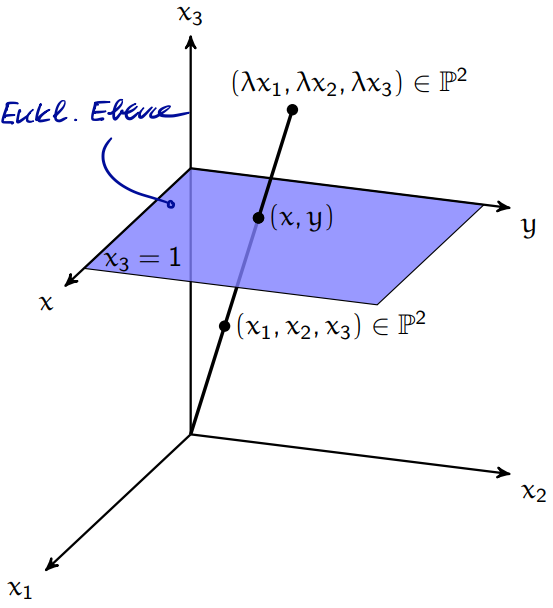
\includegraphics[width=0.24\textwidth]{assets/euclidean-plane.png}
    }
    & \textit{Ein Punkt auf der euklid-} \\
    & \textit{ischen Ebene entspricht} \\
    & \textit{dem Wert eines dehomogen-} \\
    & \textit{isierten Punktes $(x,y)$.} \\
    & \\
    & \textit{$x_3 = 1$ ergibt die} \\
    & \textit{euklidische Ebene.} \\
    & \\
    & \textit{$\lambda(x_1, x_2, x_3)$ sind Punkte} \\
    & \textit{auf einer Gerade die den Punkt} \\
    & \textit{$(\frac{x_1 \lambda}{x_3 \lambda}, \frac{x_2 \lambda}{x_3 \lambda}) = (x,y)$ definieren.} \\
\end{tabular} \\

\subsection{Projektive Transformation}

\textit{
    Abbildungen $h: \mathbb{P}^2 \mapsto \mathbb{P}^2$
    mit Eigenschaften:
}

\begin{itemize}
    \item $h$ ist eindeutig (bijektiv) und daher umkehrbar
    \item $h$ Transformationen sind geradentreu (geraden auf geraden abbilden)
    \item \textbf{Homogene Matrix} ist bis auf eine Konstante bestimmt ($k\mathbf{H} = \mathbf{H}$; $k > 0$)
\end{itemize}

$\vec{r}' = h(\vec{r}) = \mathbf{H} \vec{r}$, $\mathbf{H} = \begin{bmatrix}
    h_{11} & h_{12} & h_{13} \\
    h_{21} & h_{22} & h_{23} \\
    h_{31} & h_{32} & h_{33} \\
\end{bmatrix}$

\subsection{Transformationen kombinieren}

$\vec{r} ' = h(\vec{r}) = (h_2 \circ h_1)(\vec{r}) = h_2(h_1(\vec{r}))$\\

$\mathbf{H} = \mathbf{H}_2\mathbf{H}_1$,
$\vec{r} ' = \mathbf{H}\vec{r} = \mathbf{H}_2 \cdot \mathbf{H}_1\vec{r}$

\textit{\\
    $h_1: \mathbb{P}^2 \mapsto \mathbb{P}^2$,
    $h_2: \mathbb{P}^2 \mapsto \mathbb{P}^2$ \\
    $h = h_2 \circ h_1$ entspricht erst $h_2$ dann $h_1$
}

\subsection{Translation 2D}

$\vec{r} ' = \left[\begin{array}{cc|c}
    1 & 0 & t_x \\
    0 & 1 & t_y \\
    \hline
    0 & 0 & 1 \\
\end{array}\right]
\vec{r} = \mathbf{T} \vec{r}$ \\

\textit{Verschiebung durch $\vec{t} = \begin{bmatrix}
    t_x \\
    t_y \\
\end{bmatrix}$, $\mathbf{T}^{-1}$ entspricht $-\vec{t}$ in $\mathbf{T}$}

\subsection{Nullpunkt Rotation 2D}

$\vec{r}' = \left[\begin{array}{cc|c}
    \cos(\phi) & -\sin(\phi) & 0 \\
    \sin(\phi) & \cos(\phi) & 0 \\
    \hline
    0 & 0 & 1 \\
\end{array}\right] = \mathbf{R} \vec{r}$

\textit{Rotation mit $\phi$, $\mathbf{R}^{-1}$
entspricht $\sin$ vertauschen}

\subsection{Rotation um Punkt $A$}

\textit{Punkt: $A(t_x, t_y)$}

\begin{enumerate}
    \item Translation $A$ zum Nullpunkt verschiebt ($\mathbf{T}$)
    \item Nullpunkt Rotation 2D mit Winkel $\Phi$
    \item Translation $A$ zurück ($\mathbf{T}^{-1}$)
\end{enumerate}

$\mathbf{R} = \mathbf{T}^{-1} \mathbf{R}_0 \mathbf{T} = \begin{bmatrix}
    1 & 0 & t_x \\
    0 & 1 & t_y \\
    0 & 0 & 1 \\
\end{bmatrix} \begin{bmatrix}
    \cos(\Phi) & -\sin(\Phi) & 0 \\
    \sin(\Phi) & \cos(\Phi) & 0 \\
    0 & 0 & 1 \\
\end{bmatrix} \begin{bmatrix}
    1 & 0 & -t_x \\
    0 & 1 & -t_y \\
    0 & 0 & 1 \\
\end{bmatrix}$

\subsection{Spiegelung mit Gerade durch Ursprung}

\begin{tabular}{cl}
    \multirow{8}{*}{
        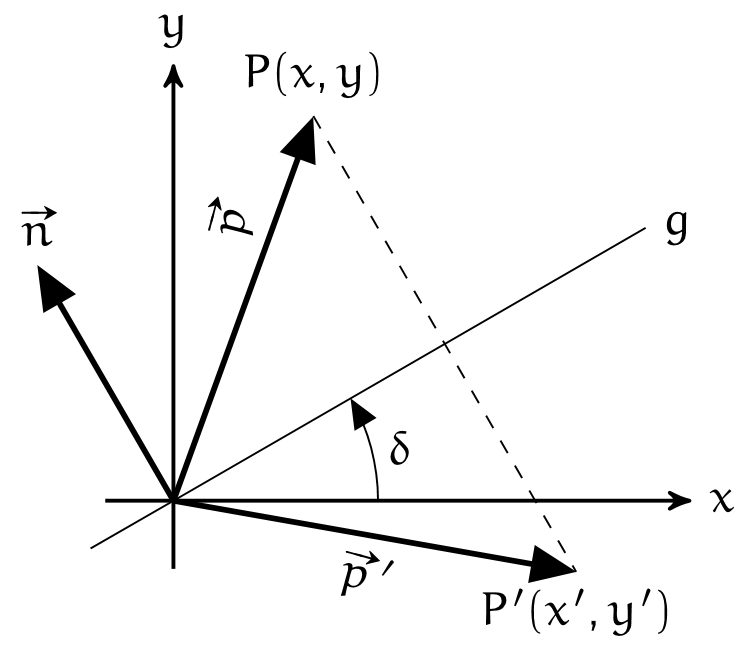
\includegraphics[width=0.2\textwidth]{assets/mirror-on-line.png}
    } & $\vec{n} = (-\sin(\delta), cos(\delta))^T$ \\
    & \\
    & HNF: $-\sin(\delta)x + cos(\delta)y = 0$\\
    & \\
    & $\vec{p}' = \vec{p} - 2 (\vec{p} \bullet \vec{n}) \vec{n}$\\
    & \\
    & $\delta = \arctan(\frac{y}{x})$ \\
    & \textit{Wenn $g$ geht durch Nullpunkt}\\
\end{tabular}

$\vec{r}' = \left[\begin{array}{cc|c}
    \cos(2\delta) & \sin(2\delta) & 0 \\
    \sin(2\delta) & -\cos(2\delta) & 0 \\
    \hline
    0 & 0 & 1 \\
\end{array}\right] \vec{r}$

\subsection{Spiegelung mit Gerade $g$}

\begin{enumerate}
    \item gerade ins Zentrum Transformieren ($\mathbf{T}$ errechnen)
    \item Spiegelung mit Gerade durch Ursprung ($\mathbf{S}$)
    \item zurück Transformieren ($\mathbf{T}^{-1}$)
\end{enumerate}

$\mathbf{M} = \mathbf{T^{-1}ST}$

\subsection{Transformation des Koordinatensystemes}

$ \begin{bmatrix}
    \cos(-\Phi) & -\sin(-\Phi) & 0 \\
    \sin(-\Phi) & \cos(-\Phi) & 0 \\
    0 & 0 & 1 \\
\end{bmatrix}$

\textit{Rotation des Koordinatensystemes um $\Phi$}

\textit{Bei einer Transformation des Koordinatensystemes
handelt es sich um eine Inverse Matrix der normalen
Transformation}

\subsection{Transformationen 2D}

$t=\begin{bmatrix}
    x \\
    y \\
\end{bmatrix}$, $0^T = \begin{bmatrix}
    0 \\
    0 \\
\end{bmatrix}$, $\mathbf{RMC} =$ 2x2 Matrix

\textbf{Euklidisch} (starre Bewegung) \\
$D = \begin{bmatrix}
    \mathbf{R} & t \\
    0^T & 1
\end{bmatrix}$ \\
\textit{Abstand zwischen zwei Punkten, alle Winkel} \\
\textit{($R^{-1} = R^T$)} \\

\textbf{Ähnlichkeit} \\
$S = \begin{bmatrix}
    k \cdot \mathbf{M} & t \\
    0^T & 1
\end{bmatrix}$ \\
\textit{Winkel zwischen zwei Punkten, alle Winkel} \\

\textbf{Affin} \\
$A = \begin{bmatrix}
    \mathbf{C} & t \\
    0^T & 1
\end{bmatrix}$ \\
\textit{Parallelität, Verhältnis zwischen Flächeninhalte} \\

\textbf{Allgemein} \\
$\mathbf{H} = \begin{bmatrix}
    h_{11} & h_{12} & h_{13} \\
    h_{21} & h_{22} & h_{23} \\
    h_{31} & h_{32} & h_{33} \\
\end{bmatrix}$ \\
\textit{Geraden bleiben Geraden} \\
